\section{Моделирование робота}
\subsection{ZenCad}
В качестве CAD программы для моделирования деталей робота и создания цифрового двойника была выбрана библиотека параметрического 3d моделирования ZenCad. Автор библиотеки вдохновлен программой OpenScad, проектирование в котором заключалось в написании скрипта, являющегося инструкцией для графического ядра, строящего модель. Без интерактивных инструментов изменения объектов. В ZenCad используется ядро граничного представления OpenCascade, что является преимуществом по сравнению с OpenScad, использующим математику полигональных сеток. Необходимость представлять каждую модель, как массив полигонов приводит к комбинаторному взрыву, при усложнении сцены, что в свою очередь заставляет разрабатывать модели с меньшим разрешением, чем их финальный вид, ради экономии вычислительных ресурсов. Особенностью граничного представления твёрдого тела заключается в описании модели, как набора поверхностей, с заданной точностью соединенных по границам и образующих замкнутый объем. То-есть окружность задается не как многоугольник с заданным количеством вершин, а именно как функция окружности, задаваемая двумя точками: центром и точкой на окружности, соответствующей 0 радиан. Подобное представление позволяет определять объем тела и его массово-инерционные характеристики, а также упрощает его разбиение на конечные элементы для инженерного анализа (так как можно легко определить, лежит ли точка внутри тела или за его пределами). Для удобства работы параметрические модели представляются в виде логического дерева построения. Фактически, каждая геометрическая операция (вытянуть, построить по сечениям и др.) – это набор алгоритмов, создающих набор корректно связанных поверхностей. При изменении компонента дерева построения все последующие элементы будут перестроены. Если при этом исчезнут элементы, к которым были привязаны последующие построения, то модель окажется некорректной. Поэтому, проектируя изделие, необходимо четко представлять иерархию дерева и возможные способы последующего изменения геометрии.

Для ускорения расчетов сцены используется библиотека ленивых вычислений evalcache для агрессивного кэширования вычислений. Это дает несколько преимуществ. Во-первых, расчеты внутри программы будут происходить только в том случае, если потребовался результат этих вычислений. Например, если объект не используется в конечной сцене, он не будет обсчитан. Во-вторых, объекты, параметры которых не были изменены будут исключены из расчетов, а данные о них загружены из кэша, где храняться предыдущие вычисления. В том числе и одинаковые объекты сцены не будут обсчитаны несколько раз. Ради демонстрации моделей с разными значениями параметров, можно заранее их обсчитать и соответственно разные версии модели будут храниться в кэше. В теории возможно переносить папку кэша с одного компьютера на другой, если это целесообразно (очень сложный проект и маломощный компьютер). С другой стороны, моделирование в ZenCad представляет собой программирование, то-есть изменение текстового документа, для чего возможно использовать любой компьютер и текстовый редактор.

Созданный мной цифровой двойник написан на языке <<Python>>, который является скриптовым языком. Это обозначает, что язык не имеет собственного компилятора, а программы представляют собой скрипт. Скрипт - это записанная в виде текста последовательность команд, которые будет выполнять интерпритатор Python, при условии, если он сможет обнаружить все неообходимые для выполнения библиотеки. Текст моего проекта разделён на четыре логических секций:

\paragraph{Константы} здесь размещены все константы, используемые в скрипте и их часто используемые отношения, для облегчения расчетов и экономии места.
\paragraph{Функции} для удобства работы с деталями робота, все они создаются в виде функций, к которым происходит обращение в нужный момент. К некоторым функциям, бывают обращения внутри других функций, например, для выреза под гайку, которая используется в нескольких деталях.  
\paragraph{Файлы STL} Так как целью проекта являтся создание физического макета, детали которого будут напечатаны на 3д принтере, то существует специальный раздел, где собраны все функции, создающие STL файлы. STL - это широкоиспользуемый формат для обмена 3д моделями в виде готовой полигональной сетки. Данный формат не подходит для дальнейших преобразований моделей (кроме линейного масштабирования). Это удобно тем, что автор, не желающий выдавать секреты проектирования своей модели, может разместить в открытом доступе конечный результат, с которым возможно работать, только  как с законченной моделью. В частности, напечатать на 3д принтере. К слову, создание проектов в ZenCad заключается в написании текста, а значит попадают под законодательство об авторском праве, что тоже может быть немаловажно для определенных задач.
\paragraph{Интерактивные объекты и анимация} особенностью ZenCad является то, что сами по себе модели не будут присутствовать в сцене до тех пор, пока не будут превращены в интерактивные объекты. Чрезвычайно глобальное отличие от OpenScad, что можно создавать различные сцены и привязывать к ним интерактивные объекты, при этом объекты, не задействованные в создании интерактивных объектов, не будут обсчитаны совсем.

Есть несколько способов создания интерактивных объектов, я использую функцию n = disp(m) (сокращение от Display), которая из объекта, хранящейся в переменной m, создает интерактивный объект n. Отличие объекта от интерактивного объекта можно рассмотреть на примере создания анимации. Если координату куба представить в виде массива из 10 значений, а после создать из него интерактивный объект, то мы увидим, как в сцене будет сгенерировано 10 кубов. Для создания анимации движения, необходимо менять координату именно интерактивного тела, что делается с помощью специальных преобразований. 


\subsection{Ласточкин хвост (Создание произвольного полигона)} 
В проекте несколько раз используется крепление типа <<Ласточкин хвост>>, для создания которого используется возможность построения многоугольника polygon по массиву точек pnts, состоящего из координат точек. В приведенной ниже функции, первым шагом происходит проверка флага f на True/False, что символизирует будет ли данных объект непосредственно ласточкиным хвостом или пазом под него. Это важно, так как паз должен иметь зазор, определяемый переменной dh. Зазор подобран экспериментально, напечатанные детали имеют достаточно шершавые поверхности, в следствие послойного наплавления. При данном зазоре одна деталь с трудом стыкуется с другой и держится силой трения. При объявлении двумерного массива pnts, вносятся координаты в формате $[[x_{1},y_{1}] , [x_{2},y_{2}]]$, которые автоматически воспринимаются как 2 координаты Х и У, фигура соответственно получается плоской и в плоскости ХУ. Если бы стояла задача использовать все три координаты их можно было записывать как $[[x_{1},y_{1},z_{1}] , [x_{2},y_{2},z_{2}]]$. После получения плоской фигуры (трапеции), происходит ее экструдирование с помощью функции linear\_extrude() на вектор vec=(0,0,20).         

\begin{lstlisting}[style=python,caption=Создание полигона из массива точек]
    def hvost(f): # Ласточкин хвост
        if f == 1 :
            dh = 0.3
        else:
            dh = 0
        pnts=      [[ 20 + dh , 10  + dh],
                    [ 10 + dh , -10 - dh],
                    [-10 - dh , -10 - dh],
                    [-20 - dh , 10  + dh]]
        o=polygon(pnts=pnts,wire=False)
        m=linear_extrude(proto=o,vec=(0,0,20),center=True)
    return m
\end{lstlisting}
\subsection{База (Создание моделей и булевы операции)}

База представляет собой основную конструкционную часть робота, задающей конструкционную жесткость для всех остальных элементов конструкции. Основной сложностью для  создания дельта робота, заключается в необходимости с большой точностью располагать рычаги под углом в $120^{\circ}$ друг к другу. От точности углов, чрезвычайно сильно зависит возможность управления роботом в дальнейшем. К счастью, 3д печать, как и ЧПУ фрезеровка, позволяет обойти эту сложность, убирая человеческий фактор, так как расположение всех креплений и отверстий задается станком с высокой точностью. В следствие моего решения печатать все детали робота на 3д принтере, я обязан уместить их в рамках печатной поверхности своего принтера, а именно в квадрат 20х20 сантиметров. В проекте присутствует дополнительное построение (квадрат из красных линий), обозначающий размер печатного стола принтера. Так как база не умещается в данные габариты, мне пришлось сделать ее разборной. Центральная цилиндрическая часть имеет 3 паза под ласточкин хвост, в которые встают "лепестки" с креплением для двигателей, червячного редуктора, концевиков и оси рычага.

\paragraph{Вырез под гайку} позволяет упростить процесс сборки и симпатично спрятать гайки внутри конструкции. Сам по себе, он имеет форму шестигранного цилиндра. Для создания шестигранника используется специальная функция ngon() с параметром n (количество граней) равным шести. Параметр wire отвечает за то, является ли двумерный объект полноценным, заполненным полигоном или только контуром. Основная сложность остается в определении радиуса. В данном случае подразумевается радиус описанной окружности многоугольника. Если измерить гайку штангель-циркулем, то получится диаметр вписанной окружности шестиугольника. Так как в шестиугольнике радус описанной окружности относится к радиусу вписанной как $sin(60^{\circ})$, получаем соотношение:

\begin{center}
    $r_{ngon} = \frac{0.5*2}{\sqrt{3}}*d_{gaika} + dh_{zazor}$
\end{center}

Итоговая величина зазора подбиралась экспериментально, чтобы гайка входила в гнездо плавно и не выпадала под собственным весом. Конкретно $dh=0.225$. Стоит отметить, что подобная подгонка имеет смысл, когда деталь печатается шестигранным отверстим к верху, когда оно свободно от поддержек или не деформировано, как любое небольшое горизонтальное отверстие.  

\begin{lstlisting}[style=python,caption=Линейная развертка (эксрудирование)]
    def pos_gaiki(): # функция выреза под гайку
        m = ngon(r=4.15,n=6,wire=False)
        n = linear_extrude(proto=m, vec=(0,0,5), center=True)
    return n
\end{lstlisting}

\paragraph{Центральная часть робота} помимо скрепления "лепестков" также имеет важную функцию крепления дельта-робота к его рабочему месту. В данном случае, так как стояла задача создания макета робота, была создана легкая рама из алюминиевого квадратного профиля, непосредственно стыкуемого с центральным элементом робота. В его рабочей версии, крепление придется значительно переработать.

Для нейро-сетевого процесса управлением роботом, в базе предусмотрено посадочное место для расположения камеры точно по центру.  
 
\begin{figure}[h!]
\centering
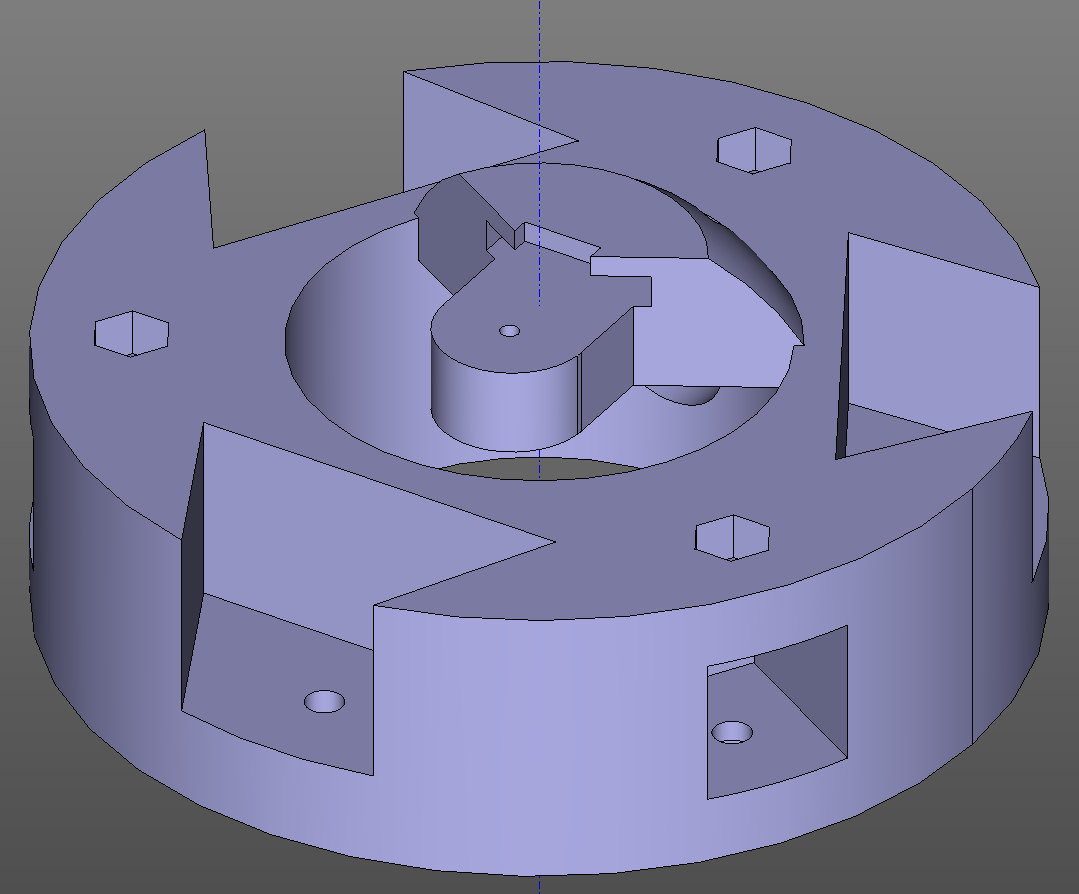
\includegraphics[width=0.8\linewidth]{./image/baza}
\caption{Центральная деталь дельта-робота}
\end{figure} 

Все крепления осуществляются винтами М4 с шляпками под внутренний шестигранник и самоконтрящимися гайками.

\paragraph{Лепесток} отвечает за один из важнейших параметров дельта-робота, а именно за радиус базы, переменную rad. Изменение радиуса базы (расстояние от центра робота, до одной из осей вращения рычагов) меняется за счет изменения длины данной детали. В данном случае, предоставлено значение rad = 150 милиметров, которое можно считать предельным значением. Минимальным значением можно считать 90 миллиметров, если не менять конфигурацию центральной части. При значениях меньше 90 мм., целесообразно печатать базу единой деталью.   

\begin{figure}[h!]
\centering
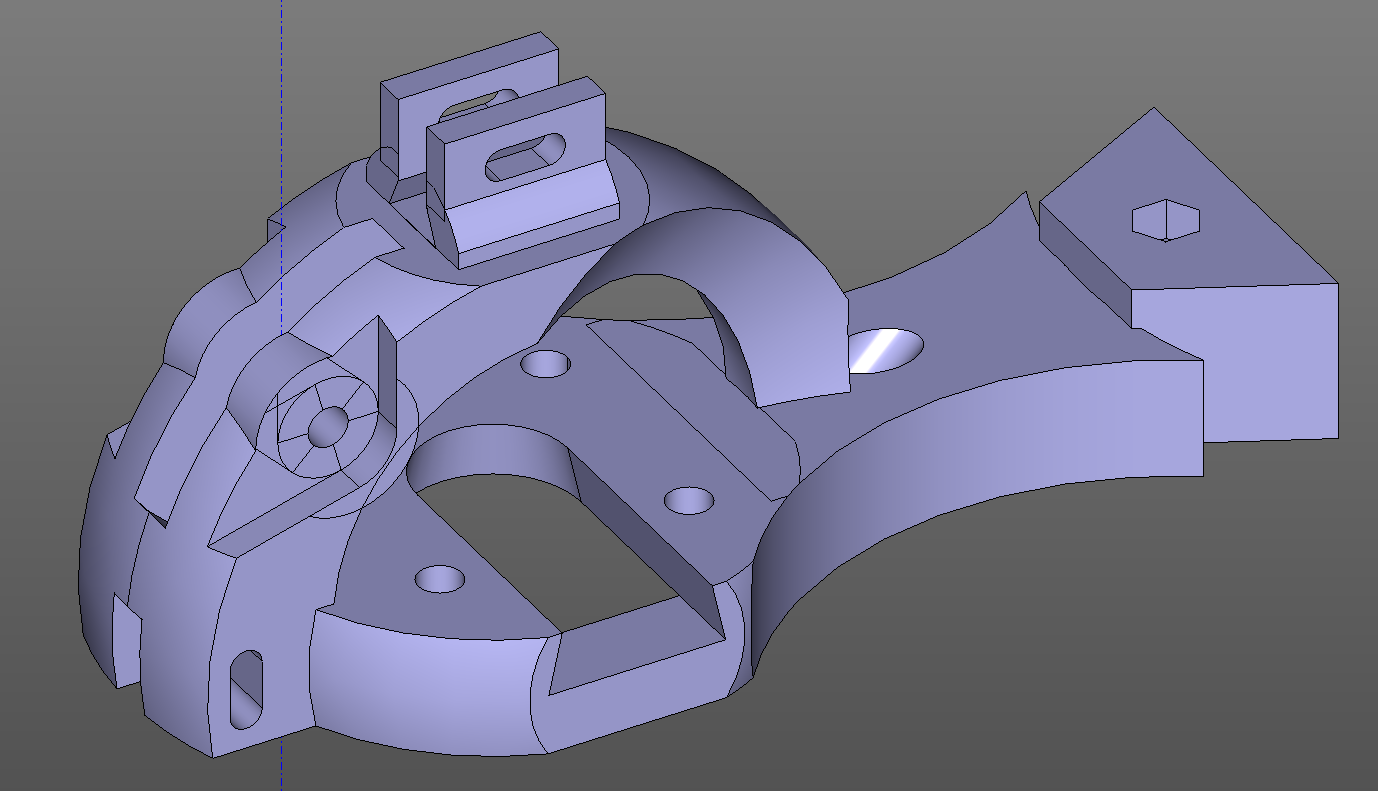
\includegraphics[width=0.8\linewidth]{./image/lepestok}
\caption{Вторая деталь базы дельта-робота}
\end{figure} 

Для увеличения жесткости напечатанной детали, желательно придавать ей как можно больше сложных криволинейных поверхностей. В данном случае использовано максимальное количество сферических поверхностей. Все прямоугольные поверхности проектировались по принципу пересечения сферы с кубом, или вычитания сфер из формы. 

\begin{lstlisting}[style=python,caption=Булева операция пересечения]
     krep = box((xz_dvig+20,xz_dvig+20,15),center=True)\
            ^ sphere(r=0.8*xz_dvig)
\end{lstlisting}

В частности главная центральная часть данной детали (крепеж шагового двигателя), это прямоугольный параллелепипед со сторонами Х и У на 20 миллиметров больше, чем габариты двигателя, и  Z стороной равной 15 мм. С помощью оператора $\wedge$ находится пересечение со сферой радиусом 80 $\%$ от величины габаритов двигателя. Таким образом вместо прямоугольных форм получаются округлые,  способные противостоять большим скручивающим нагрузкам. Расположенная перпендикулярно арка также представляет собой полусферу, пересеченную с кубоидом. Пространство под аркой представляет собой вычтенную сферу, так как располагающийся там глобоидный червь тоже имеет габариты сферы. В следствие этого, края арки находятся немного ниже высоты червя, и тот на свое место встает с щелчком, за счет упругости пластика. Это один из способов удержания червя, использованный тут.

У каждого лепестка есть два настраиваемых крепления для концевиков, позволяющие немного регулировать крайние положения рычага. При настройке робота крайне важно выставить рычаги в начальные позиции (в моем случае это $-15^{\circ}$) и для облегчения настройки, есть физическое ограничение для поворота рычага соответствующие положениям $-15^{\circ}$ и $90^{\circ}$. Таким образом, выставив рычаг в одно из крайних положений, есть возможность отрегулировать позицию концевика на срабатывание в нужный момент. 

\subsection{Глобоидная червячная передача (Параллельные вычисления)}

Глобоидная червячная передача является разновидностью червячных передач, когда зона механического соприкосновения червя и колеса изогнута по вогнутой (глобоидной) траектории. Это обеспечивает большое сцепление по количеству зубьев в несколько раз (в сравнении с цилиндрическим червем) в зависимости от конфигурации количества зубьев и диаметра колеса. В промышленных механизмах данная передача используется редко из-за некоторых минусов, связанных со сложностью изготовления и настройки глобоидной передачи. Также её характерной особенностью является повышенное тепловыделение, а следовательно повышенный износ и сниженный КПД, в сравнении с цилиндрическим червём. Тем не менее, в данной конструкции глобоидная передача позволит в небольшом объеме сделать пластиковый редуктор с максимально большими зубьями у рабочих колес. Максимально возможный размер зубьев, подразумевает возможность повысить надежность пластиковой конструкции и упростить требования к печати деталей.  

\paragraph{Двумерное шестеренчатое колесо} является необходимым элементом, для выбранного мной способа моделирования червя. Идея построения заключается в том, чтобы взять некую форму заготовки (цилиндр или в моем случае полусферу) и, поворачивая ее вокруг своей оси, вычесть из нее форму шестеренчатого колеса, которая при этом сама поворачивается вокруг собственной оси. Таким образом, можно быть точно уверенным, что моделируемый червь и колесо идеально подходят друг к другу.

Поэтому, в первую очередь, предстояло выбрать форму шестеренчатого колеса. Самая простая форма для зубьев (если не рассматривать процесс изготовления, а с точки зрения воображения) это зубья сферической формы. Рассмотрим функцию построения двумерной шестерни из окружностей. Так как необходимые значения шага резьбы и количества зубьев изначально не определены, функция должна генерировать шестерню с произвольными значениями этих переменных. Данные две переменные являются одними из основных и вынесены в первый блок проекта. Называются teeth (количество зубов зубчатого колеса) и step (шаг резьбы червячной передачи). 
\vspace{0.5cm}

\begin{figure}[h]
\centering
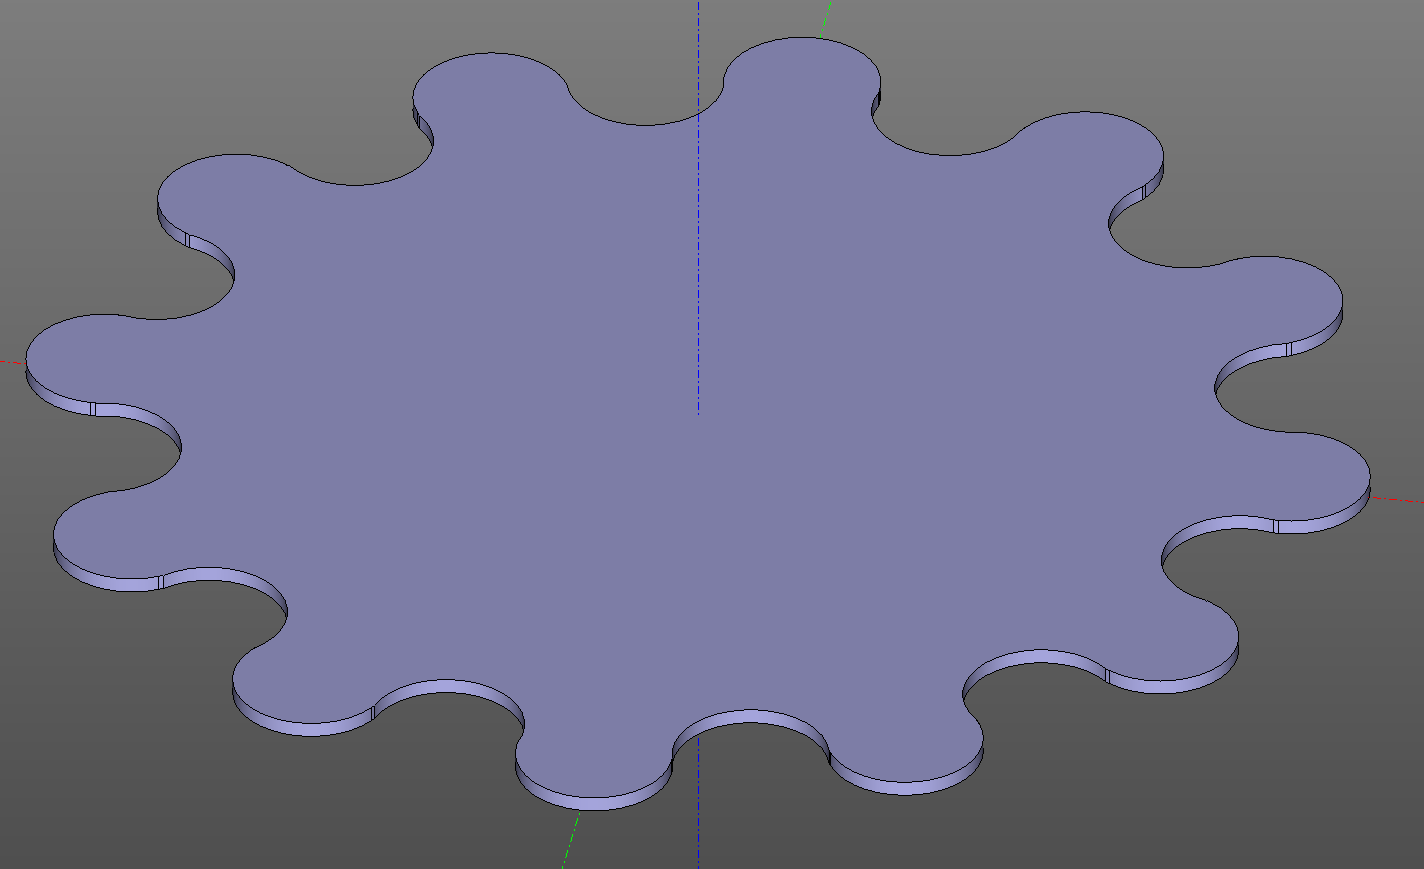
\includegraphics[width=0.65\linewidth]{./image/gear}
\caption{Пример работы функции (добавлен объем)}
\end{figure} 

\begin{lstlisting}[style=python,caption=Работа с линиями объединение]
def gear(teeth,step): # Функция шестерни
    angle = pi/teeth
    a  = i*2*angle
    rad_opis = (step/2) / math.sin(angle/2)
    rad_vpis = (step/2) / math.tan(angle/2)
    c=[]
    def c1(i): # Функция зуба колеса
        c1 = circle(step/2,angle=(1.5*pi,0.5*pi), wire=True)\
            .moveX(rad_opis).rotateZ(a)
        return c1
    def c2(i): # Функция впадины колеса
        c2 = circle(step/2,angle=(0.5*pi,1.5*pi), wire=True)\
             .moveX(rad_vpis).rotateZ(a+angle)
        return c2
    for i in range(teeth):
        o = sew([c1(i),\
    segment(c1(i).endpoints()[-1],c2(i).endpoints()[-1]),\
                c2(i)  ])
        p = segment(c2(i).endpoints()[0],\
        c1(i+1).endpoints()[0])
        c.append(o)
        c.append(p)
    return sew(c)
\end{lstlisting}

Основная задача данной функции заключается в том, чтобы расставить половинки окружностей определенным образом в пространстве. Для формирования формы шестеренчатого колеса, можно представить многоугольник в вершинах которого расположены центры окружностей зубьев, а серединах сторон - центры окружностей, вырезающие впадины. Количество вершин многоугольника будет соответствовать количеству зубьев колеса (teeth), а сторона - шагу резьбы (step). 

Внутри функции объявлены две отдельные функции c1(i) и c2(i) для построения i-той половинки окружности зуба и впадины соответственно. А внутри них располагается функция circle(), которая имеет 3 параметра: радиус окружности, угол (angle), с помощью которого создается не окружность целиком, а дуга, ограниченная начальным и конечным углом, и wire - является объект контуром или сегментом. Радиус окружностей равен половине шага резьбы. Чтобы поместить цент окружности во все вершины многоугольника, нужно один раз сместить его на радиус описанной окружности и teeth раз повернуть на удвоенный угол angle. Таким образом используется удобство полярных координат. Для впадин аналогично, но переместить нужно на радиус вписанной окружности. Оба радиуса и угол находятся с помощью тригонометрии в самом начале.

Самое сложное в данной функции - это получение из разрозненных кусочков, единый двумерный объект. Для соединения нескольких линий в одну, существует функция sew([line1,line2]), которая обрабатывает массивы, состоящие из линий. Соответственно, необходимо объявить массив c=[] и циклично добавлять в него полуокружности, чтобы потом объединить их в единое целое. К сожалению, в месте, где должны соединяться полуокружности рядом находится большое количество точек, и алгоритм функции sew() не способен самостоятельно решить, какие точки необходимо скреплять, поэтому ему необходимо помочь. Необходимо воспользоваться функцией segment(point1, point2), которая создает отрезок, соединяющий точки point1 и point2. В качестве точек нужно взять граничные точки линий, для чего существует преобразование line.endpoints()[0], где 0 - это номер точки объекта line. Конечно, таким образом можно обратиться к любой точке, из которой состоит линия, но как обратиться к последней точке? Так как линия является массивом из точек, то задача состоит в обращении к последнему элементу массива, номера которого мы не знаем. В python мы можем это сделать, вызвав переполнение, то-есть обратившись к -1 элементу массива.

В контексте данной задачи, линия O представляет собой сумму зуба, впадины и отрезка, соединяющих их последние точки. Линия P представляет собой отрезок, соединяющий первую точку впадины с первой точкой следующего зуба. Когда цикл teeth раз добавит эти линии к массиву с, будет возможно полностью объединить массив в одну линию и вернуть ее, как результат работы функции - return sew(c). Обращаю внимание, что алгоритм делает все операции за один цикл 

В данном случае явно продемонстрированы сложности, связанные с тем, что ZenCad использует ядро граничного представления. В случае с OpenScad мелкие погрешности несовпадения точек в пространстве, были бы нивелированы, представлением окружностей, как многогранников с четко определенными величинами минимальных деталей. В ZenCad даже ничтожный разрыв линии превратит замкнутую фигуру в незамкнутую, за чем необходимо очень пристально следить. Так как к незамкнутым фигурам нельзя применить те операции, которые необходимо сделать в дальнейшем.

\paragraph{Создание тора из вращающейся шестерни}  Если взять полученную выше шестерню и замкнуть её в трёхмерный тор, параллельно поворачивая её вокруг своей оси, то можно получить форму, обратную форме червя. Достаточно будет вычесть этот тор из сферы или цилиндра, чтобы получить конечную форму глобоидного червя. Задача состоит в том, чтобы разработать алгоритм построения данной фигуры и, так как её расчёт будет достаточно затратным для вычислительных мощностей, распараллелить вычисления, благо python предлагает инструменты для этого. 

Идея создания фигуры заключается в том, чтобы построить выше смоделированную шестерню, сдвинуть ее от центра на радиус будущего тора. Следующую построить аналогично, но при этом повернуть по оси Z относительно центра на угол "b" и одновременно повернуть ее вокруг собственной оси на угол "a". При этом переменная "n" отвечает за детализацию будущей фигуры. Переменная "n\_s" отвечает за количество оборотов, которое сделает шестерня, пройдя всю окружность по тору. Это очень важная переменная, так как от  нее зависит не гладкость поверхности, а передаточное число червячной передачи. "n\_s" задает количество зубьев на теле червяка, в моем проекте это три восходящие спирали. Данное решение сильно уменьшает передаточное число, что положительно сказывается на скорости робота, но при этом такой червяк плохо стопорит шестерню и в некоторых позициях возможна передача движения со стороны шестерни. То-есть по мере увеличения количества зубьев у червя, передача превращается в экстравагантно выглядящую угловую зубчатую передачу. Но самое главное, что в небольшом объеме, мы можем создать зубчатые колеса с очень большими зубьями, которые просто напечатать на 3д принтере и износостойкость, которых будет велика за счет отсутствия мелких (меньше 4 мм.) деталей. 

Для распараллеливания вычислений используется модуль futures. Идея заключается в том, чтобы фигуру, похожую на тор, разделить на 4 равные части и рассчитывать эти части параллельно в 4 потока. Поэтому в начале функции вставлена проверка значения переменной х, от которой зависят переменные da и db - начальный сдвиг углов a и b соответственно. Функция chast(x) в зависимости от х будет строить четвертинку итоговой фигуры и её необходимо запустить 4 раза. В данном случае, ThreadPoolExecutor() создает пул из количества потоков, равному количеству элементов в массиве х, а именно 4 потока, внутри которых будет выполняться функция chast() со своим значением переменной х. Более элегантным решением было бы в массив х занести значения одного из углов сдвига, а второй считать через формулу, это позволит отказаться от части с проверкой и легко менять количество потоков, редактированием массива. В данном случае нельзя изменить количество потоков, без правки проверок внутри функции chast().   


\begin{figure}[h]
\centering
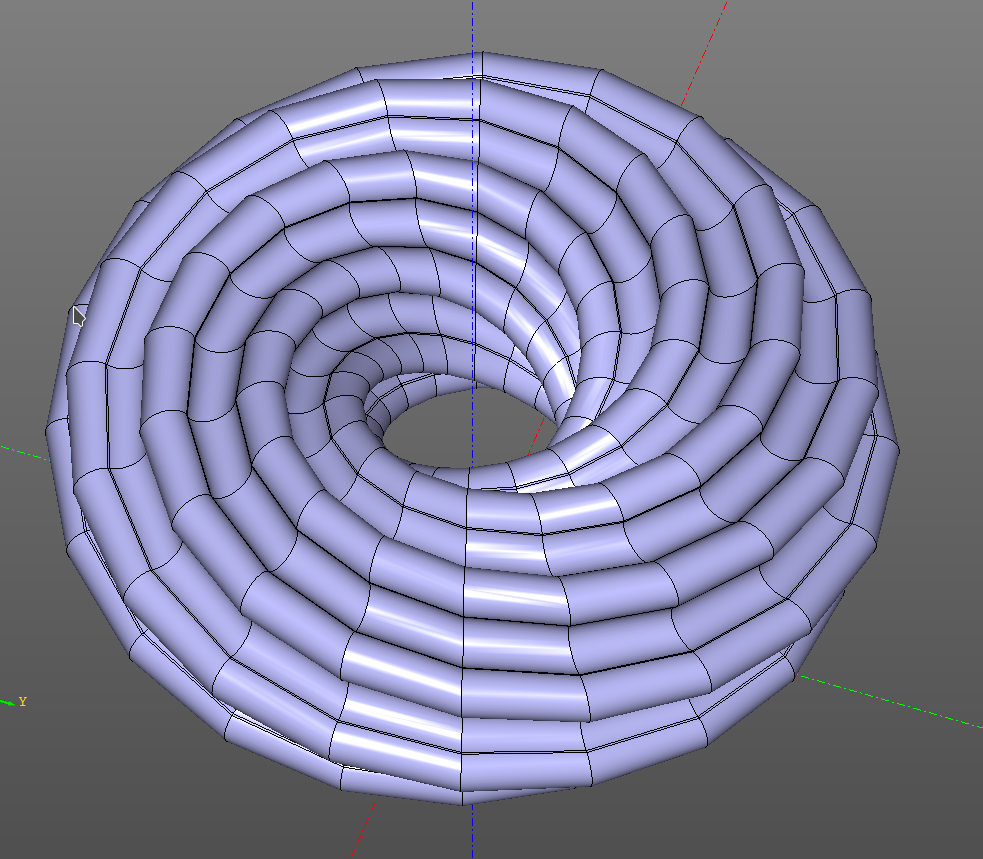
\includegraphics[width=0.8\linewidth]{./image/worm_tor}
\caption{Обратная форма глобоидного червя}
\end{figure}

После получения обратной формы червя, нужно взять фигуру-заготовку цилиндр или полусферу и вычесть из нее эту форму, что не является ресурсоемкой операцией и происходит мгновенно. Остается только добавить некоторые дополнительные детали червя: отверстие под вал двигателя с прямоугольным скосом, отверстие для отвертки, позволяющее прикрутить двигатель с надетой шестерней и конусный <<ласточкин хвост>>, дополнительно фиксирующий червя в пазу. Для уменьшения вероятности того, что вал провернется в теле червя, предусмотрено место для запрессовывания специальной латунной зубчатой гайки, которая крепится к валу двигателя винтом. С червем она соприкасается зубьями и держится за счет трения. 

\newpage
\begin{lstlisting}[style=python,caption=Код функции создающей червя]
from concurrent import futures
def worm (): # Червь
    angle = pi/teeth
    rad_opis =(step/2) / math.tan(angle/2)
    a = (n_s*angle*0.5)/n
    b = 0.5*pi/n
    def chast(x):  # выбор четверти в зависимости от х
        if x==
                da = 0
                db = 0
        if x==1:
                da = a*n
                db = pi/2
        if x==2:
                da = 2*a*n
                db = pi
        if x==3:
                da = 3*a*n
                db = 1.5*pi
        g=[]
        r=0.5*(xz_dvig+10)
        for i in range(n+1):  # цикл расстановки двумерных шестеренок 
                g.append(gear(teeth,step).rotateY(i*a + da)\
                            .translate(r,0,20).rotateZ(i*b + db))
        w = loft(g) # "обтягивание" двумерных фигур  
        return w
    x = [i for i in range(0,4,1)]   # создание и запуск 4 потоков
    with futures.ThreadPoolExecutor() as executor: 
        worm = executor.map(chast, x)
    o = cylinder(r=3,h=30,center=True).up(15)\ #отверстие под вал  
        ^cube([6,6,20],center=True).translate(1,0,10)
    w = sphere(r=0.5*(xz_dvig+10),pitch=(0,pi/2))\ # полусфера
        - union(list(worm))\  # объединенный в 1 объект тор
        - cylinder(2,50,True).translate(0.5*otverstia,0.5*otverstia,0)
    w = w - o + cone(r1=10.4, r2=9.2, h=6,center=True).down(3)\
          - cylinder(11.2/2,11,True).down(0.5)\
          - cylinder(1.5,12,True).rotateY(deg(90))\
          .translate(-5,0,-5.5+2.7)
    return w.rotateZ(deg( 90)).rotateY(deg(180))
 \end{lstlisting}
 
\paragraph{Объемная шестерня} для ее создания, как это ни странно, не используется функция gear(). Для плавного скольжения по желобам червя, зубья шестерни должны иметь форму сферы. Плоской шестеренку можно сделать только при небольшой толщине, в пару мм. при больших значениях она перестает вставляться в червя. При сферической форме зуба толщину шестеренки можно приравнять к шагу резьбы, тем самым сделав её массивной и достаточно прочной. 

\subsection{Вспомогательные модели (Сборочные юниты)}

К вспомогательным построениям можно отнести вещи, добавленные в сцену ради визуального наполнения. К ним относятся модель платы arduino с дополнением cnc shield v3. Не смотря на то, функционально данная модель только показывает габариты и расположение отверстий крепления, при моделировании возникли сложности. ZenCad в его сегодняшнем исполнении, не подразумевает наличия у моделей текстуры или цвета. Функцию color() возможно применить только к интерактивным объектам сцены, привязав каждому объекту конкретный цвет. Как же тогда создать разноцветную модель, или как перемещать сборную модель, объединяющую детали разных цветов, как единое целое? Необходимо обратиться к сборочным юнитам.

Сборочный юнит - это объект, имеющий собственную локальную систему координат, относительно которой позиционируются связанные с этим юнитом интерактивные объекты и другие юниты. Их следует структурировать в виде дерева, отсчитывая  положение относительно положения юнита-предка (unit.parent). Если юнит не имеет предка, его положение отсчитывается от глобальной системы координат.
Юнит содержит имеет два объекта координатного преобразования - location и global\_location. 

Location - задаёт положение юнита относительно положения юнита предка. location может быть обновлён или непосредственно, или с помощью метода relocate.
globallocation - это положение юнита относительно глобальной системы координат. globallocation используется при отрисовке объекта. globallocation строится на основе дерева unit.location и может быть обновлён с помощью метода locationupdate, relocate и, с помощью других операций.

Конечно, смысл объединения объектов в древовидное древо, не создание разноцветных моделей, а удобное размещение их в пространстве сцены. Мы вынуждены каждый элемент определенного цвета создавать отдельно, но имеем возможность манипулировать ими, как группой. К такой группе могут быть примененны все афинные преобразования, в том числе и масштабирование.

\begin{figure}[h]
\centering
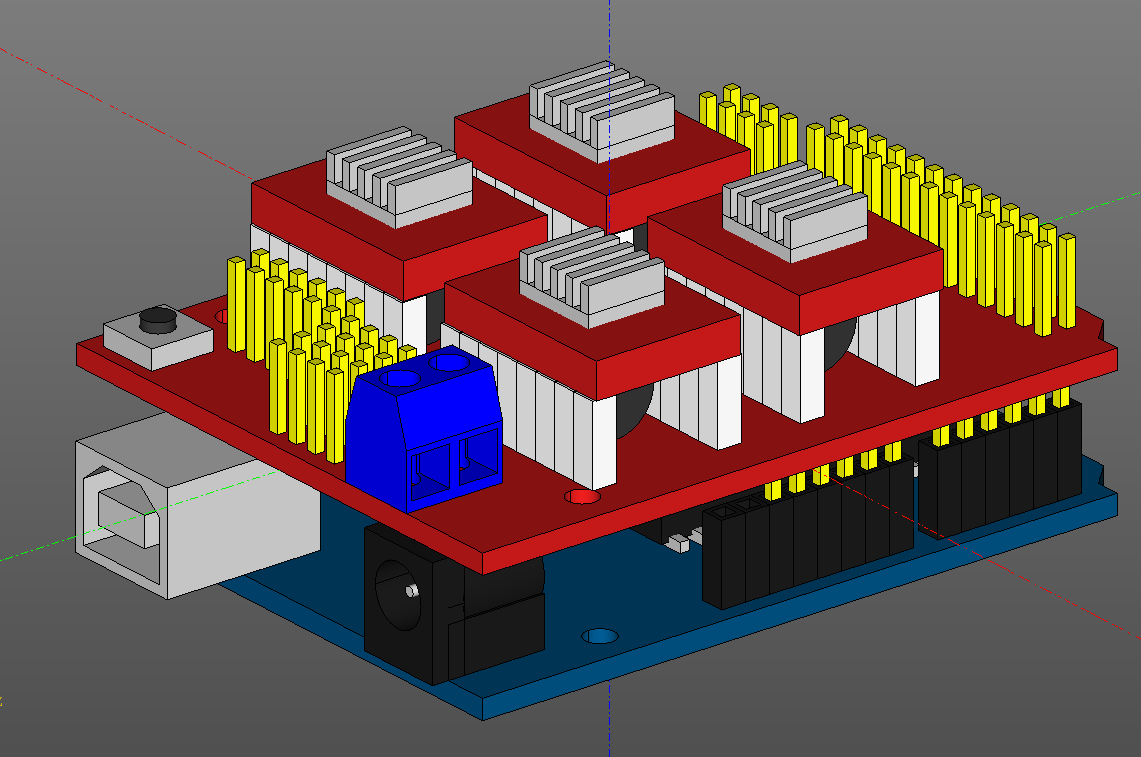
\includegraphics[width=0.8\linewidth]{./image/arduino}
\caption{Модель платы Arduino cnc shield v3}
\end{figure}



 \begin{lstlisting}[style=python,caption=Пример сборочного юнита]
arduino = zencad.assemble.unit()
arduino.add_shape(plate(1), color(0,0.31,0.5))
arduino.add_shape(usb(), color(0.8,0.8,0.8))
arduino.add_shape(pit(), color(0.1,0.1,0.1))
arduino.add_shape(pit2(), color(0.8,0.8,.8))
arduino.add_shape(knopka(), color(0.8,0.8,.8))
arduino.add_shape(knopka2(), color(0.8,0.2,0.2))
arduino.add_shape(micro(), color(0.1,0.1,0.1))
arduino.add_shape(micro2(), color(0.8,0.8,0.8))
arduino.add_shape(raz1(), color(0.1,0.1,0.1))

shild = zencad.assemble.unit()
shild.add_shape(plate(0),color(0.8,0.1,0.1))
shild.add_shape(shtik(),color.yellow)
shild.add_shape(knopka(), color(0.8,0.8,.8))
shild.add_shape(knopka2(), color(0.2,0.2,0.2))
shild.add_shape(kleim(), color.blue)
shild.add_shape(raz2(),color.white)
shild.add_shape(kond(), color(0.2,0.2,0.2))
shild.add_shape(drivers(),color(0.8,0.1,0.1))
shild.add_shape(radiators(), color(0.8,0.8,.8))

arduino.relocate(moveZ(-12.5))
disp(shild)
disp(arduino)
\end{lstlisting}

В качестве примера показываю, как объединял плату arduino и плату shild  в два сборных юнита, состоящих из набора функций, строящих определенные элементы, наполняющие плату. К слову, функция plate(), отрисовывающая кусок текстолита, имеет логический флаг 0 или 1, отвечающий за количество отверстий в платах, так как оно разное. Строка arduino.relocate(moveZ(-12.5) * rotateY(deg(90))) перемещает  и вращает систему координат для юнитов, зависимых от предка arduino, поэтому их расположение относительно друг друга не меняется.  

Таким же методом были созданы концевики, состоящие из двух частей. 

\subsection{Движение каретки (Создание анимации)}

Последняя треть проекта оставлена под создание объектов сцены с помощью функции disp() (сокращение от display). По умолчанию display добавляет интерактивный объект в главную сцену, но есть возможность создавать различные сцены, прикреплять юниты к ним и позже отобрать командой show(). 

Объекты разделены на две группы: неподвижные и подвижные.
\paragraph{Неподвижные объекты сцены} имеют конкретную позицию относительно глобальной системы координат, которая рассчитывается один раз, до следующего изменения глобальных параметров дельта-робота. На данный момент, все они зависят от размера радиуса базы (rad). 

\begin{lstlisting}[style=python,caption=Растановка объектов методом полярных координат]
disp(krepej().moveY(-rad),color(1,0.4,0))
disp(krepej().moveY(-rad).rotateZ(deg( 120)),color(1,0.4,0))
disp(krepej().moveY(-rad).rotateZ(deg(-120)),color(1,0.4,0))
\end{lstlisting}
 
 На самом деле, формула расчета координат сложнее, но все константы я оставил внутри функции, а глобальные переменные использовал здесь. Самой главной идеей было разместить геометрический центр модели krepej в точке, где находится ось рычага. Тогда перемещение на константу rad, поместит ось рычага в необходимую точку. 
 
 \paragraph{Подвижные объекты сцены} собраны в отдельную функцию animate(widjet). Все вычисления внутри функции зависят от переменной t, которая отсчитывает время анимации. Для изменения переменной во времени используется библиотека time. 
 
\begin{lstlisting}[style=python,caption=Работа со временной переменной]
import time

nulltime = time.time()

def animate(widget):
    t = (20*(time.time() - nulltime))%210
    if (t<105):
        teta1 = t-15
        teta2 = t-15
        teta3 = t-15
    else:
        teta1 = 210-t-15
        teta2 = 210-t-15
        teta3 = 210-t-15
\end{lstlisting}

Функция time.time() возвращает текущее время, выраженное через количество секунд, прошедшее с 1 января 1970-го года. Чтобы не работать с этим большим числом, а начать отсчитывать с нуля вводится начальная точка отсчета nulltime. При каждом последующем вызове функции времени, из неё будет вычитаться начальное время. Но на самом деле, в данном случае, это ни на что не влияет и можно опустить, так как для вычисления t используется операция \%210 (нахождение остатка от деления на 210). Моей задачей было менять углы отклонения рычагов робота в их крайних пределах, а именно от $-15^{\circ}$ до $90^{\circ}$. Если считать перемещение на один градус за один такт, то движение в одну строну будет равным $15+90=105$ тактам. Добавляем движение назад и получаем $105*2=210$ число тактов на всю анимацию. Так как время течет не останавливаясь, программа будет отрабатывать анимацию циклично до конца своей работы. Коэффициент 20 перед скобкой отвечает только за скорость анимации. Так как ядро отрисовывает объекты много чаще раза в секунду, а функция времени возвращает миллисекунды, в качестве тысячных секунды, анимация не становится прерывистой от ввода коэффициента. По сути, ядро не ограничивает нас в скорости анимации. Ради эксперимента можно попробовать заставить объект вращаться со скоростью, кратной герцовки экрана монитора и добиться стробоскопического эффекта. Ниже пример программы, где я заставляю тело вращаться со скоростью 589.95 оборотов в секунду, превратив propeler в мигающий, но почти неподвижный восьмелистник. При небольшом изменении частоты, кажущееся направление вращения меняет свое направление, по часовой или против часовой стрелки. Число 589.95 не кратно 60 Гц экрана, так как очевидно есть задержки, необходимые процессору для вычислений и на разных компьютерах придется подбирать свою частоту вращения. 
\begin{lstlisting}[style=python,caption=Стробоскопический эффект на экране монитора]
from zencad import * 
import time 
 
m=box((100,10,10),center=True) 
 
propeler = disp(m) 
 
def animate(widget): 
    t = (589.95*time.time())%36 
    propeler.relocate(rotateY(deg(10*t))) 
   
show(animate=animate)
\end{lstlisting}

Для создания анимации необходимо понимать разницу между объектами и интерактивными объектами. Можно попробовать создать объект, координата которого зависит от времени. Тогда мы увидим, как каждый такт создаются копии этого объекта, которые постепенно заполняют сцену. Потому что мы создали интерактивный объект, состоящий из размножающихся во времени объектов. Данный прием я использую для рисования траектории движения каретки, в качестве объекта используя точку (point(X,Y,Z)). 

\begin{lstlisting}[style=python,caption=Рисование максимальных траекторий дельта-робота]
def animate(widget):
    t = (20*(time.time() - nulltime))
    k = 105
    d = 120 #20*t/360
    p = 15

    teta1= k*math.fabs(math.sin(deg(t))) - p
    teta2= k*math.fabs(math.sin(deg(t - d))) - p
    teta3= k*math.fabs(math.sin(deg(t + d))) - p

\end{lstlisting}

В качестве демонстрации движения, я придумал такой небольшой алгоритм, где углы отклонения рычагов меняются по синусоидальному закону, и имеют сдвиг по фазе относительно друг друга (d).
С помощью параметров k и p задается диапозон значений [-15:90].
Функция fabs возвращает модуль от синусоиды, чтобы избавиться от отрицательных значений, которое здесь не нужны.  
Если сделать сдвиг по фазе равный $120^{\circ}$, то можно добиться максимальных отклонений: когда один рычаг будет в минимальной позиции, два других будут в максимальных и наоборот.
Если сдвиг по фазе будет с разными знаками, как в примере выше, то мы увидим максимальную по радиусу круговую траекторию, на которую способен робот.
Если знаки у сдвига будут одинаковыми, то мы увидим максимальное боковое смещение каретки.
На рисунке траектории обозначены чёрной линией.
Можно отметить, что граница рабочей зоны дельта-робота имеет в горизонтальном сечении треугольную форму, что следует учитывать при расположении робота на его рабочем месте.  

\begin{figure}[h]
\centering
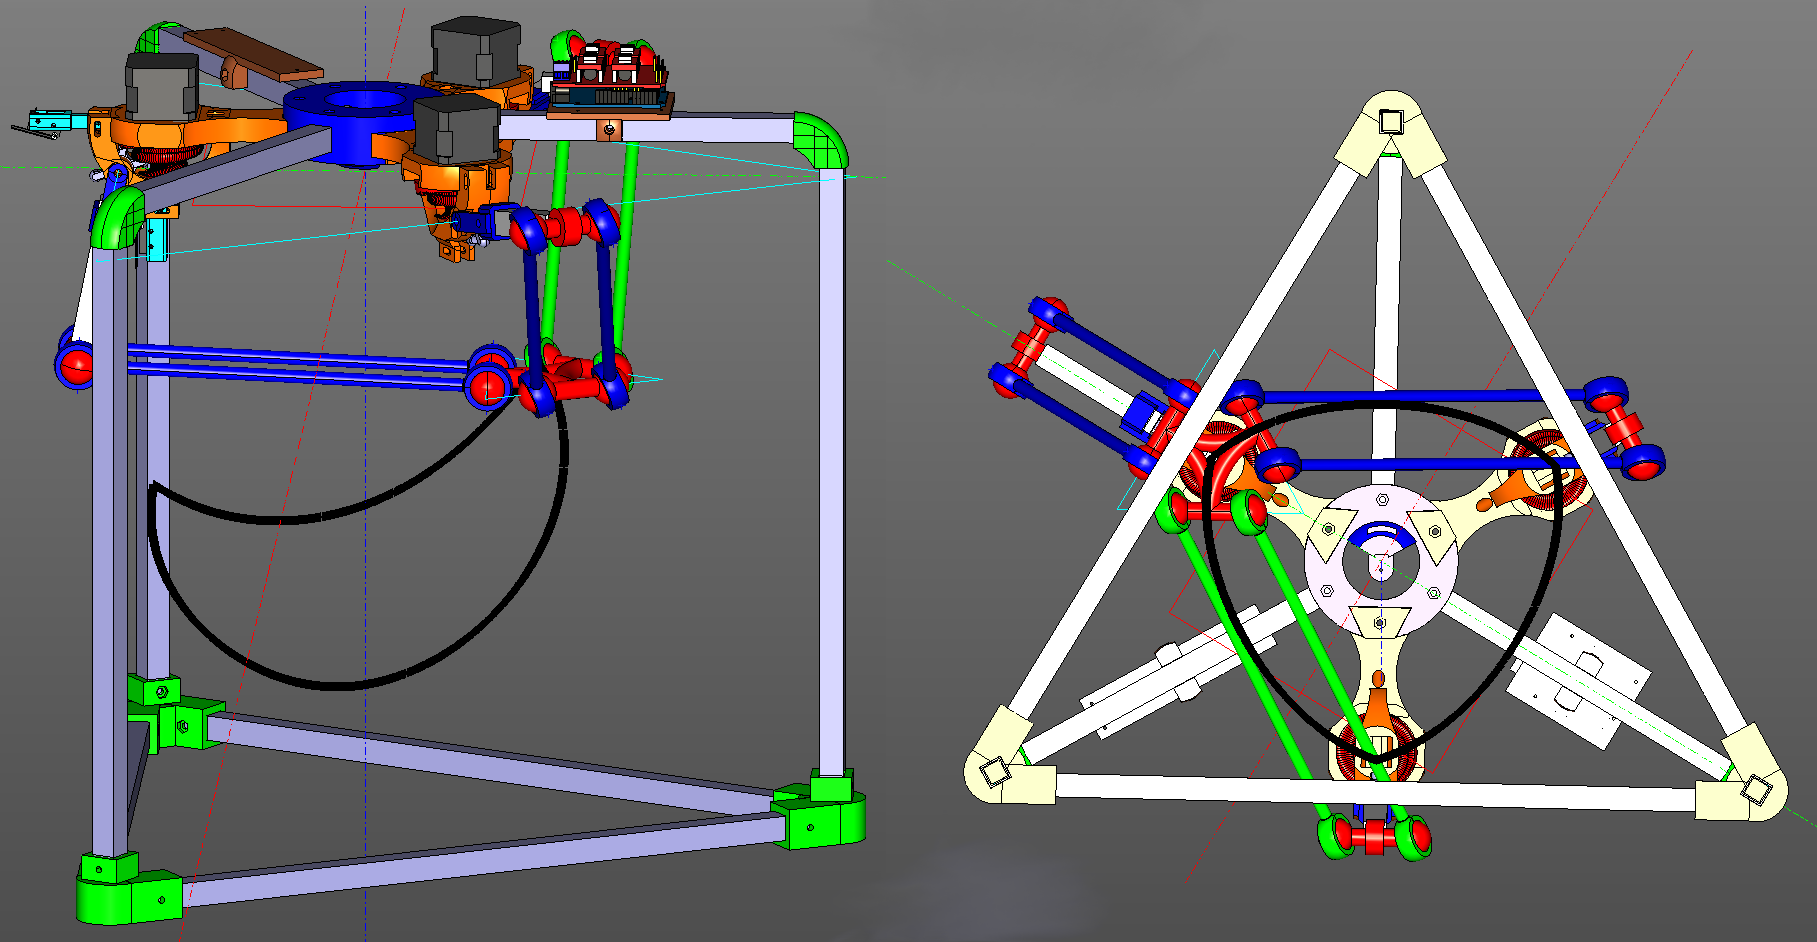
\includegraphics[width=0.8\linewidth]{./image/traek}
\caption{Максимальные траектории движения дельта-робота }
\end{figure}


\subsection{Расчет координат и углов объектов (Вращение координат)}

\paragraph{Простые вычисления.} Рассмотрим пример размещения первой группы анимированных объектов. Это именно те объекты, положение которых меняется в одной плоскости и его возможно напрямую (в одно действие) рассчитать из углов $\theta_{i}$. А именно червяка, шестеренки, рычага и верхней части локтя (часть шарнира карданного крепления). 
\begin{lstlisting}[style=python,caption=Простые анимированные объекты]
#========1 рука
worm1.relocate(translate(0,-rad+rich_x,19.5) *  rotateZ(deg(-3*teta1 )))
gear3d1.relocate(moveY(-rad) * rotateX(deg(teta1)))
plecho1.relocate(moveY(-rad) * rotateX(deg(teta1)))
plecho_krep1.relocate(moveY(-rad) * rotateX(deg(teta1)))
lokot_verh1.relocate(moveY(-rad) * rotateX(deg(teta1)))
#========2 рука
worm2.relocate(translate(1.732*0.5*(rad-rich_x),0.5*(rad-rich_x),19.5)\
    * rotateZ(deg(-3*teta2 + 120)))
gear3d2.relocate(translate(1.732*0.5*rad,0.5*rad,0)\
    * rotateZ(deg(120)) * rotateX(deg(teta2)))
plecho2.relocate(translate(1.732*0.5*rad,0.5*rad,0)\
    * rotateZ(deg(120)) * rotateX(deg(teta2)))
plecho_krep2.relocate(translate(1.732*0.5*rad,0.5*rad,0)\
    * rotateZ(deg(120)) * rotateX(deg(teta2)))
lokot_verh2.relocate(translate(1.732*0.5*rad,0.5*rad,0)\
    * rotateZ(deg(120)) * rotateX(deg(teta2)))  
#========3 рука
worm3.relocate(translate(-1.732*0.5*(rad-rich_x),0.5*(rad-rich_x),19.5)\
    * rotateZ(deg(-3*teta3 - 120)))
gear3d3.relocate(translate(-1.732*0.5*rad,0.5*rad,0)\
    * rotateZ(deg(-120)) * rotateX(deg(teta3)))
plecho3.relocate(translate(-1.732*0.5*rad,0.5*rad,0)\
    * rotateZ(deg(-120)) * rotateX(deg(teta3)))
plecho_krep3.relocate(translate(-1.732*0.5*rad,0.5*rad,0)\
    * rotateZ(deg(-120)) * rotateX(deg(teta3)))
lokot_verh3.relocate(translate(-1.732*0.5*rad,0.5*rad,0)\
    * rotateZ(deg(-120)) * rotateX(deg(teta3)))
\end{lstlisting}

Если присмотреться к данному отрывку кода, то можно заметить общее единообразие в том, как происходит размещение объектов. В первой руке происходит сдвиг по Y координате на -rad (иногда встречается отступ rich\_x, который зависит от форм-фактора двигателя), и поворот на угол $\theta_{1}$. У второй и третьей руки все происходит аналогично, но добавляется поворот по Z на $120^{\circ}$ и $-120^{\circ}$ соответственно и некие коэффициенты 1.732 и 0.5. На самом деле координаты деталей второй и третьей руки рассчитываются по формуле вращения координат.
\begin{center}
\begin{align}
&x_{2}=x_{1}\cos{(120^{\circ})} + y_{1}\sin{(120^{\circ})} \nonumber\\
&y_{2}=-x_{1}\sin{(120^{\circ})}+ y_{1}\cos{(120^{\circ})} \nonumber\\
&x_{3}=x_{1}\cos{(-120^{\circ})}+ y_{1}\sin{(-120^{\circ})} \nonumber\\
&y_{3}=-x_{1}\sin{(-120^{\circ})}+ y_{1}\cos{(-120^{\circ})} \nonumber
\end{align}
\end{center}

 Как видно вторая и третья рука строятся аналогичным образом, что и первая, только через преобразование координат по формуле вращения системы координат, относительно оси Z. Но это только размещение на нужной координате, при этом объект остается повернутым, относительно своей новой системы координат. Ему требуется поворот вокруг собственной оси на $120^{\circ}$, для выравнивания со своей новой системой координат. Поэтому и появляется во второй и третьей руке дополнительная функция rotateZ(deg(120)). Можно отметить, что здесь заложено, что скорость вращения червяка в 3 раза больше, скорости вращения остальных деталей.
 
 \paragraph{Вычисления прямой задачи управления.} Вторая группа анимированных деталей поворачиваются, следуя за кареткой, либо непосредственно присоедененны к ней. Поэтому вычисление их положения, невозможны без вычисления координат каретки. Вычисляются они по формулам, приведенным в главе про кинематику.
 
\begin{lstlisting}[style=python,caption=Решение прямой задачи управления дельта-робота]
t = rad - 0.5*E  # радиус вписанной окружности

x1 = 0
y1 = -rad + e  - Rf*math.cos(deg(teta1))
z1 = -Rf*math.sin(deg(teta1))

x2 = (-rad + e - Rf*math.cos(deg(teta2)))*math.sin(deg(120))
y2 = (-rad + e - Rf*math.cos(deg(teta2)))*math.cos(deg(120))
z2 = -Rf*math.sin(deg(teta2))

x3 = (-rad + e - Rf*math.cos(deg(teta3)))*math.sin(deg(-120))
y3 = (-rad + e - Rf*math.cos(deg(teta3)))*math.cos(deg(-120))
z3 = -Rf*math.sin(deg(teta3))

dnm = (y2-y1)*x3-(y3-y1)*x2

w1 = y1**2 + z1**2
w2 = x2**2 + y2**2 + z2**2
w3 = x3**2 + y3**2 + z3**2

a1 =  (z2-z1)*(y3-y1) - (z3-z1)*(y2-y1)
b1 = -( (w2-w1)*(y3-y1) - (w3-w1)*(y2-y1) )/2

a2 = -(z2-z1)*x3 + (z3-z1)*x2
b2 = ((w2-w1)*x3 - (w3-w1)*x2)/ 2

a = a1**2 + a2**2 + dnm**2
b = 2*(a1*b1 + a2*(b2-y1*dnm) - z1*dnm**2)
c = (b2-y1*dnm)**2 + b1**2 + (dnm**2)*(z1**2 - Re**2)

d = b**2 - 4*a*c
Z = -0.5*(b + math.sqrt(d))/a
X = (a1*Z + b1)/dnm
Y = (a2*Z + b2)/dnm

\end{lstlisting}

В конце этих вычислений получаются координаты $(X,Y,Z)$, которые присваиваются каретке и определяют её конечное положение в пространстве.

\paragraph{Карданное соединение (векторная алгебра).} Вычисления выше начинаются с расчета координат $(x_{i},y_{i},z_{i})$, которые являются координатами локтей (обозначены красным цветом на рис. 8). Но локти были расставлены уже до этого другим методом. Сложность возникает с карданным крепежом (обозначен синим цветом на рис. 8), который в проекте обозначен, как arm1p. Где цифра обозначает номер руки робота, а <<p>> и <<l>> - <<правая>> и <<левая>>. Всего их шесть штук. Задача заключается в том, чтобы по двум координатам (координате локтя и каретки) рассчитать положение в пространстве каждой из arm.  

\begin{figure}[h]
\centering
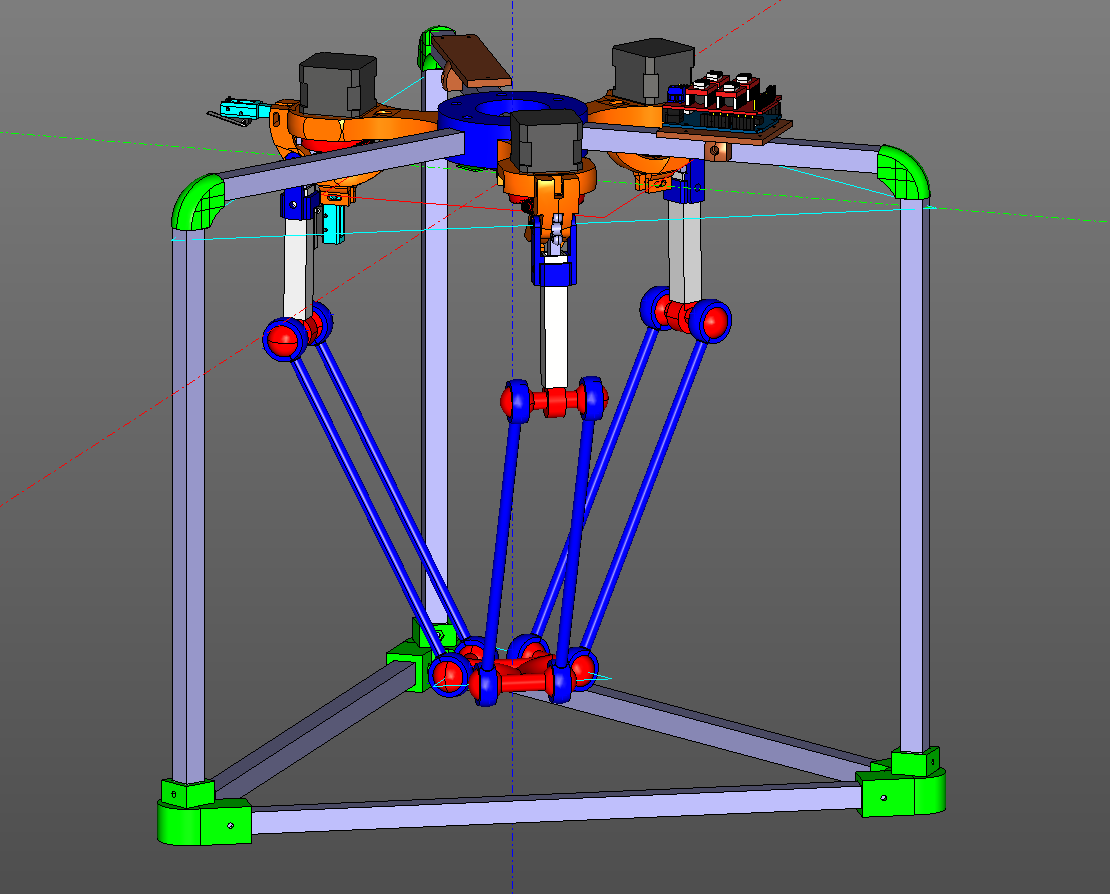
\includegraphics[width=0.8\linewidth]{./image/arm}
\caption{Общий вид дельта-робота}
\end{figure}

Arm состоит из верхнего и нижнего кольца, охватывающих сферу шарнира и трубки их соединяющих. Функция строит arm таким образом, чтобы центр верхнего кольца был в начале координат. Поэтому первоначальное расположение будет соответствовать координатам $(x_{i},y_{i},z_{i})$, со смещением вправо или влево. Остается повернуть его в двух плоскостях таким образом, чтобы нижнее кольцо <<наделось>> на шарнир каретки. В случае с первой рукой координата для нижнего кольца легко рассчитывается из $(X,Y,Z)$. Каретка не поворачивается в пространстве, при движении все её точки рисуют взаимно параллельные линии. Поэтому координаты креплений не будут меняться, если их выразить через координаты центра каретки. Рассчитав координаты верхнего и нижнего кольца и, зная расстояние между ними, так как это константа, можно рассчитать проекции угла на плоскость ZX и ZY. Соответственно рассчитав значение проекций, можно будет найти углы поворота. 

\begin{figure}[h]
\centering
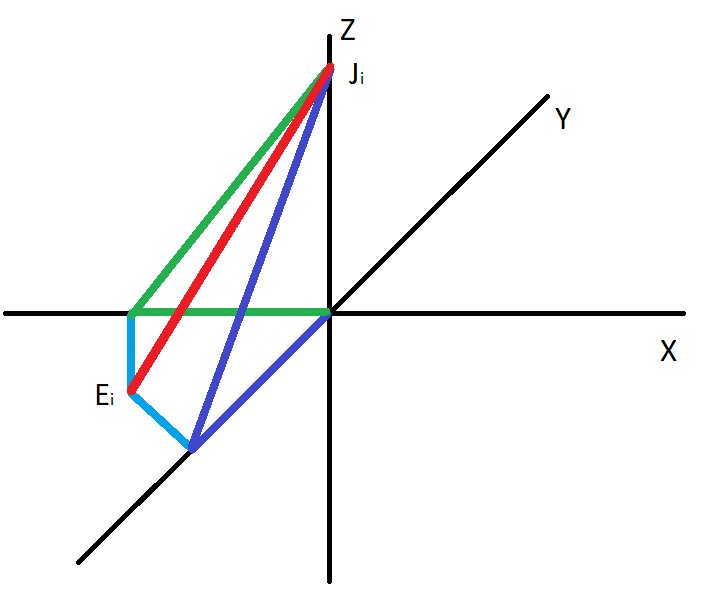
\includegraphics[width=0.6\linewidth]{./image/proection}
\caption{Проекции}
\end{figure}

Пример для первой руки:

\begin{lstlisting}[style=python,caption=Тригонометрический способ ориентирования шарниров]
arm1p.relocate(translate(x1+0.5*l_karetki,y1-0.5*E,z1)\
        * rotateY(-math.asin( (X-x1)/Re ) )\
        * rotateX(math.asin( (Y-y1)/Re ) ))
arm1l.relocate(translate(x1-0.5*l_karetki,y1-0.5*E,z1)\
        * rotateY(-math.asin( (X-x1)/Re ) )\
        * rotateX(math.asin( (Y-y1)/Re ) ))
\end{lstlisting}

К сожалению, данный метод перестал работать в нынешней версии ZenCad, так второй поворот будет происходить относительно системы координат, смещенной первым поворотом, а не относительно глобальной системы координат. Более того, очередность поворотов тоже влияет на конечный результат. Это произошло потому, что правила вращения интерактивных и обычных объектов привели к единообразию. Зато появился более правильный и простой способ повернуть карданный крепеж на требуемый угол, а именно - векторный поворот.
Ниже представлен пример векторного поворота для двух карданных креплений, соединяющих первый рычаг с кареткой. Необходимо расчитать координаты, где крепление стыкуется с локтем (точка $pN = (x_l, y_l, z_{i})$ ), и точку стыковки с кареткой $(pK = (Xk, Yk, Z))$. 

\begin{lstlisting}[style=python,caption=Векторный поворот первого шарнира]
x_l = x1 + 0.5*l_karetki
y_l = y1 - e

Xk = X + 0.5*l_karetki
Yk = Y - e

pN = point(x_l, y_l, z1)
pK = point(Xk,Yk,Z)
arm1p.relocate(translate(*pN)\
        * short_rotate(f=(0,0,-1), t=pK-pN) )


x_l = x1 - 0.5*l_karetki
y_l = y1 - e

Xk = X - 0.5*l_karetki
Yk = Y - e

pN = point(x_l, y_l, z1)
pK = point(Xk,Yk,Z)
arm1l.relocate(translate(*pN)\
        * short_rotate(f=(0,0,-1), t=pK-pN) )

\end{lstlisting}

После простого расчета координат точек, необходимо создать объект точку (point()). После чего переместить объект arm1p в точку pN, где находится его соединение с локтем. Тут использована ссылка на адрес переменной (translate(*pN)).  И вторым действием, повернуть тело arm1p на вектор t, относительно вектора f. Вектор f показывает начальное положение тела arm1p (оно направлено вертикально вниз), а вектор t - необходимая позиция. Чтобы перенести вектор t в начало координат, необходимо из координат конца вектора, вычесть коодинаты начала вектора. В итоге мы получаем, что тело arm1p своим началом находится в точке pN, а своим концом смотрит на точку pK. По большому счету, в данном примере, мы сделали тоже самое, что и в примере выше, только тригонометрические вычисления углов спрятаны внутри функции short\_rotate(). И пользователю теперь не нужно думать о тригонометрии.

В случае со вторым и третим рычагами, расчеты аналогичные, но координаты точек pN и pK расчитываются с применением приема вращения координат. 

\begin{lstlisting}[style=python,caption=Векторный поворот второго шарнира]
x_l = x2 - 0.866*e - 0.25*l_karetki
y_l = y2 + 0.5*e - 0.433*l_karetki

Xk = X - 0.866*e - 0.25*l_karetki
Yk = Y + 0.5*e - 0.433*l_karetki

pN = point(x_l, y_l, z2)
pK = point(Xk,Yk,Z)
arm2p.relocate(translate(*pN)\
        * short_rotate(f=(0,0,-1), t=pK-pN) )

x_l = x2 - 0.866*e + 0.25*l_karetki
y_l = y2 + 0.5*e + 0.433*l_karetki

Xk = X - 0.866*e + 0.25*l_karetki
Yk = Y + 0.5*e + 0.433*l_karetki

pN = point(x_l, y_l, z2)
pK = point(Xk,Yk,Z)
arm2l.relocate(translate(*pN)\
        * short_rotate(f=(0,0,-1), t=pK-pN) )
\end{lstlisting}

\subsection{Создание моделей (Экспорт в STL)}

ZenCad удобен тем, что позволяет массово экспортировать детали в нужные директории и делать это при каждом обновлении геометрии деталей. При процессе преобразования модели из объекта представлений в полигональную сетку необходимо задать минимальный размер сегментов сетки, который в данном случае составляет 0.01 миллиметра. Неудобство заключается в том, что на данный момент функция требует ввода полного пути от корня до имени файла. Нельзя указать текущюю директорию через точку или домашнюю директорию через тильду. В системе виндовс, путь прописывается аналогично, начиная с диска и заканчивая именем файла. При переносе файл в другую систему, необходимо убедиться, что прописанные в скрипте директории существуют, иначе выполнить скрипт не получится. 

\begin{lstlisting}[style=python,caption=Создание моделей STL]
def tostl():
    m1=krepej()
    m2=basa()
    m3=plecho_krep()
    m4=ugolok_verh()
    m5=ugolok_niz()
    m6=shablon()
    m7=lokot_niz()
    m8=lokot_verh()
    m9=krep_konch()
    m10=krep_konch_niz()
    m11=ploshadka(1)
    m12=ploshadka(2)
    m13=worm()
    to_stl(m1,'/home/oleg/krepej.stl',0.01)
    to_stl(m2,'/home/oleg/basa.stl',0.01)
    to_stl(m3,'/home/oleg/plecho_krep.stl',0.01)
    to_stl(m4,'/home/oleg/ugolok_verh.stl',0.01)
    to_stl(m5,'/home/oleg/ugolok_niz.stl',0.01)
    to_stl(m6,'/home/oleg/shablon.stl',0.01)
    to_stl(m7,'/home/oleg/lokot_niz.stl',0.01)
    to_stl(m8,'/home/oleg/lokot_verh.stl',0.01)
    to_stl(m9,'/home/oleg/krep_konch.stl',0.01)
    to_stl(m10,'/home/oleg/krep_konch_niz.stl',0.01)
    to_stl(m11,'/home/oleg/ploshadka1.stl',0.01)
    to_stl(m12,'/home/oleg/ploshadka2.stl',0.01)
    to_stl(m13,'/home/oleg/worm.stl',0.01)

tostl()
\end{lstlisting}

\subsection{Вывод}

После изготовления модели дельта-робота были выявлена недостаточная жесткость конструкции. <<Лепестки>>, на которых расположены двигатели, имеют явный люфт в месте сочлинения с базой, который обусловлен неправильным позиционированием пазов. На данный момент паз сделан так, что эффективно препядствует движению в горизонтальной плоскости, но при этом дает вертикальные колебания. <<Ласточкин хвост>> требуется перевернуть на $90^{\circ}$, чтобы это исправить.
Изучив движения дельта-робота, я пришел к выводу, что величина радиуса базы должна быть значительно больше. Не в пределах от 90 мм. до 150 мм., а начинаться от 150 мм. и доходить до 300 мм. При таких плечах, делать детали целиком из пластика не имеет смысла. В новом видении дизайна робота, база должна иметь металлический скелет, а пластик будет играть роль сухожилий, связывающих все прочие детали. На стоимость робота это не должно повлиять, но упростит и ускорит процесс печати.

